\documentclass[a4paper]{article}

\usepackage[toc,page]{appendix}

\usepackage[spanish]{babel}
\usepackage[utf8]{inputenc}
\usepackage{amsmath}
\usepackage{graphicx}
\usepackage{fancyhdr}
\usepackage{amsmath}
\usepackage[colorinlistoftodos]{todonotes}
\usepackage{xcolor}
\usepackage{minted}
\usepackage[font=small,labelfont=bf]{caption}
\usepackage{enumitem}

\usepackage{hyperref}

\hypersetup{
    colorlinks,
    citecolor=blue,
    filecolor=blue,
    linkcolor=blue,
    urlcolor=blue
}

\usepackage{geometry}
\geometry{a4paper}

\begin{document}
\begin{figure}
\centering
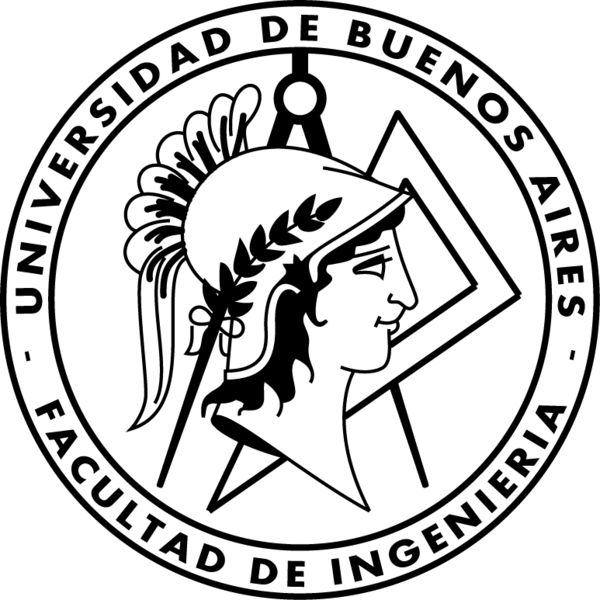
\includegraphics[scale=1]{./img/logo-facu}
\end{figure}

\title{\large\textsc{66.17 - Sistemas Digitales}\\
\large Trabajo Práctico 2 - Voltímetro digital con salida VGA}

\author{
Andrew Parlane \\
}

\maketitle

\newpage

\tableofcontents

\listoffigures

\newpage

\section{Introducción}

El objetivo de este trabajo es a diseñar, simular y implementar en FPGA un circuito digital que mide una tensión analógica y mostrarle por una pantalla VGA. El conversor A/D debe usar una entrada LVDS como un comparador para implementar un Sigma-Delta ADC.

El circuito digital debe funcionar con una Altera DE2 placa de desarrollo que tiene un cyclone II 2C35 FPGA.

\section{Herramientas}

Las herramientas que usé para este trabajo son:
\begin{itemize}[nosep]
\item Questa Sim v10.2c
\item Quartus II v13.0sp1
\item GNU Make v4.2.1
\item FTDI Font conversion utility v0.4 \url{http://www.ftdichip.com/Support/Utilities.htm}
\item SRecord v1.63 \url{http://srecord.sourceforge.net}
\item VGA Simulator \url{https://ericeastwood.com/lab/vga-simulator/}
\end{itemize}

\section{Implementación}

Los componentes principales de mi diseño son:
\begin{itemize}[nosep]
\item Contador Binario que cuenta desde cero hasta un parámetro MAX.
\item Contador BCD que cuenta desde cero hasta 99...9 con un parámetro de CIFRAS.
\item ADC Sigma-Delta que usa la entrada diferencial y una salida para obtener muestras de la señal.
\item VGA que genera las señales de VGA.
\item ADV7123 que genera las señales para uso con el ADV7123 VGA DAC.
\item Un carácter ROM que contiene las mapas de pixeles por los caracteres ASCII desde ' ' hasta '\textasciitilde'.
\item TP2 que junta todo el diseño.
\end{itemize}

\vspace{0.4cm}

También implementé unos paquetes con funcionalidad útil:
\begin{itemize}[nosep]
\item Utils para funciones genéricos y útil.
\item Type para tipos comunes.
\item VGA Timings para los timings de VGA para diferentes resoluciones.
\item Char ROM para un enum de los caracteres.
\end {itemize}

\vspace{0.4cm}

Los recursos de la placa DE2 que uso son:
\begin{itemize}[nosep]
\item Tres pins GPIO para el conversor ADC.
\item Un reloj de 50MHz.
\item Un botón para la señal reset.
\item El VGA DAC y el puerto VGA.
\end{itemize}

\vspace{0.4cm}

No voy a detallar los dos componentes de contadores aquí porque son casi el mismo del TP1. Tampoco voy a detallar los paquetes porque no son tan relevante al diseño.

\subsection{ADC}

Ese componente es Un ADC Sigma-Delta con un filtro digital low-pass. Hay un contador BCD de cinco cifras que cuenta solo cuando la entrada diferencial es un '1'. Hay un segundo contador que cuenta hasta 33001. Cuando llega a 33001 captura el valor del contador BCD, esto es la muestra. Usando un reloj de 50MHz obtenemos una muestra cada 33002 ticks = 1.5KHz.

\subsubsection{Señales y Parámetros}

\begin{tabular}{| l | l | r | l |}
\hline
\textbf{Nombre} & \textbf{Tipo} & \textbf{Bits} & \textbf{Descripción} \\ \hline
\multicolumn{4}{|c|}{Entradas} \\ \hline
clk & std\_ulogic & 1 & El reloj. \\ 
rst & std\_ulogic & 1 & Reset asíncrono. \\
dInDiff & std\_ulogic & 1 & La salida del comparador LVDS. \\ \hline
\multicolumn{4}{|c|}{Salidas} \\ \hline
dOut & std\_ulogic & 1 & dInDiff retardado un tick. \\ 
resultado & unsignedArray & 3 * 4 & La última muestra en BCD de 3 cifras. \\ \hline
\end{tabular}

\subsubsection{Diagrama de Bloques}

\begin{figure}[!h]
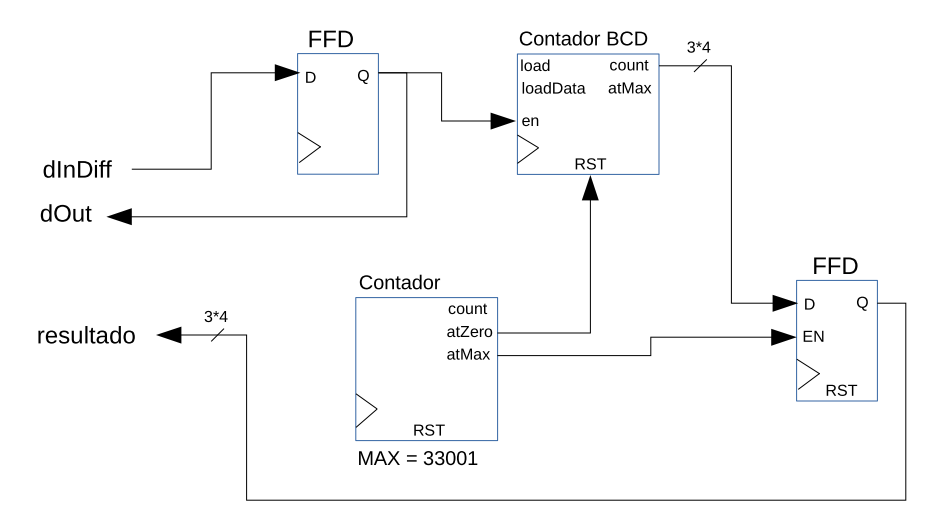
\includegraphics[width=15cm]{img/adc.png}
\captionof{figure}{Diagrama de Bloques de componente adc.}
\end{figure}

\subsection{VGA}

Ese componente genera las señales VGA hsync, vsync, un par de señales pixelX y pixelY que dicen que pixel enviamos en el siguiente tick del reloj y una señal inActive que dice si está en la región activo de la pantalla. La resolución y los timings están parámetros.

\subsubsection{Señales y Parámetros}

\begin{tabular}{| l | l | r | p{8cm} |}
\hline
\textbf{Nombre} & \textbf{Tipo} & \textbf{Bits} & \textbf{Descripción} \\ \hline
\multicolumn{4}{|c|}{Parámetros} \\ \hline
H\_ACTIVE & natural & & La resolución horizontal en pixeles. \\
H\_FRONT\_PORCH & natural & & Duración del front porch horizontal en pixeles. \\
H\_SYNC & natural & & Duración del pulso sync horizontal en pixeles. \\
H\_BACK\_PORCH & natural & & Duración del back porch horizontal en pixeles. \\
V\_ACTIVE & natural & & La resolución vertical en líneas. \\
V\_FRONT\_PORCH & natural & & Duración del front porch vertical en líneas. \\
V\_SYNC & natural & & Duración del pulso sync vertical en líneas. \\
V\_BACK\_PORCH & natural & & Duración del back porch vertical en líneas. \\ \hline
\multicolumn{4}{|c|}{Entradas} \\ \hline
clk & std\_ulogic & 1 & El reloj. \\ 
rst & std\_ulogic & 1 & Reset asíncrono. \\ \hline
\multicolumn{4}{|c|}{Salidas} \\ \hline
pixelX & unsigned & X\_WIDTH & Número de pixel activo horizontal que enviamos siguiente. \\ 
pixelY & unsigned & Y\_WIDTH & Número de pixel activo vertical que enviamos siguiente. \\ 
inActive & std\_ulogic & 1 & Ese pixel es en la región activo. \\
nHSync & std\_ulogic & 1 & La señal hsync (activo bajo). \\
nVSync & std\_ulogic & 1 & La señal vsync (activo bajo). \\
\hline
\end{tabular}

\vspace{0.5cm}
Donde X\_WIDTH es el mínimo número de bits necesarios para almacenar H\_ACTIVO, y Y\_WIDTH es el mínimo número de bits necesarios para almacenar V\_ACTIVO.

\pagebreak
\subsubsection{Diagrama de Bloques}

\begin{figure}[!h]
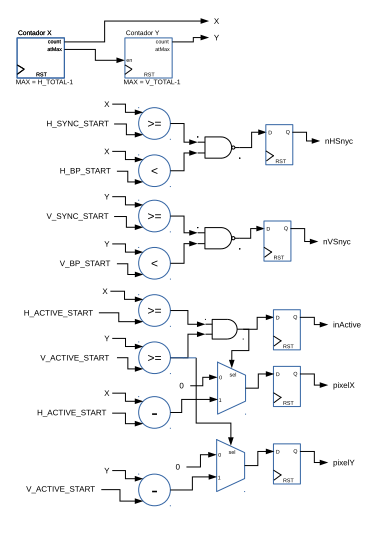
\includegraphics[width=13cm]{img/vga.png}
\captionof{figure}{Diagrama de Bloques de componente vga.}
\end{figure}

\subsection{ADV7123}

Ese componente es un wrapper del componente VGA para funcionar con el VGA DAC ADV7123.

\subsubsection{Señales y Parámetros}

Tiene todos los mismas señales de VGA más:\\ \\
\begin{tabular}{| l | l | r | p{8cm} |}
\hline
\textbf{Nombre} & \textbf{Tipo} & \textbf{Bits} & \textbf{Descripción} \\ \hline
\multicolumn{4}{|c|}{Entradas} \\ \hline
rIn & std\_ulogic\_vector & 10 & El valor rojo para el pixel pixelX. \\ 
gIn & std\_ulogic\_vector & 10 & El valor verde para el pixel pixelX. \\ 
bIn & std\_ulogic\_vector & 10 & El valor azul para el pixel pixelX. \\ 
\hline
\multicolumn{4}{|c|}{Salidas} \\ \hline
clkOut & std\_ulogic & 1 & El reloj hasta el DAC. \\
rOut & std\_ulogic\_vector & 10 & El valor rojo alineado a las otras señales. \\ 
gOut & std\_ulogic\_vector & 10 & El valor verde alineado a las otras señales. \\ 
bOut & std\_ulogic\_vector & 10 & El valor azul alineado a las otras señales. \\ 
nBlank & std\_ulogic & 1 & Igual a inActive. \\
nSync & std\_ulogic & 1 & Activo (bajo) cuando hay un pulso de hsync o vsync. \\ \hline
\end{tabular}

\subsection{ROM de caracteres}

Decidí a construir mi propio ROM de caracteres usando el font \href{https://www.fontsquirrel.com/fonts/ubuntu-mono}{Ubuntu Mono}. Usé la herramienta \textit{fnt\_cvt} para convertir el .ttf hasta la data de pixeles crudo con 1 bit cada pixel. Después usé la herramienta \textit{srec\_cat} para convertir el binario hasta un .mif. Ese data es almacenado en el block RAM del FPGA usando un \textit{Altera Mega Wizzard component}. Cada palabra del ROM es 16 bits que es el ancho de un carácter. Así cada carácter comienza con la fila igual al número de carácter multiplicado por la altura de la carácter.

\subsubsection{Señales y Parámetros}

\begin{tabular}{| l | l | r | p{8cm} |}
\hline
\textbf{Nombre} & \textbf{Tipo} & \textbf{Bits} & \textbf{Descripción} \\ \hline
\multicolumn{4}{|c|}{Entradas} \\ \hline
clk & std\_ulogic & 1 & El reloj. \\ 
rst & std\_ulogic & 1 & Reset asíncrono. \\
char & charRomCharacter & 1 & El carácter querido. \\
offX & unsigned & 4 & La pixel querido en la fila corriente. \\
offY & unsigned & 5 & La fila querido en la carácter corriente. \\
\hline
\multicolumn{4}{|c|}{Salidas} \\ \hline
px & std\_ulogic & 1 & El pixel querido. \\
\hline
\end{tabular}

\subsection{TP2}

Ese componente es el más alto que junta todo los demás. Uso una resolución de 800x600 divido en bloques de 32*16 pixeles, usando los bits mayores del pixelX y pixelY como índices al bloque, y los menores para el offset en la cuadra. A final hay un poco lógica a especificar que carácter necesita dibujar en cada bloque.

\subsubsection{Señales y Parámetros}

\begin{tabular}{| l | l | r | p{8cm} |}
\hline
\textbf{Nombre} & \textbf{Tipo} & \textbf{Bits} & \textbf{Descripción} \\ \hline
\multicolumn{4}{|c|}{Entradas} \\ \hline
CLOCK\_50 & std\_ulogic & 1 & El reloj de 50MHz. \\ 
KEY & std\_ulogic\_vector & 1 & Una botón para el reset. \\
DATA\_VOLT\_IN\_DIFF & std\_ulogic & 1 & La entrada LVDS. \\
\hline
\multicolumn{4}{|c|}{Salidas} \\ \hline
DATA\_VOLT\_OUT & std\_ulogic & 1 & La salida al red RC. \\
VGA\_R & std\_ulogic\_vector & 10 & El componente rojo del pixel. \\
VGA\_G & std\_ulogic\_vector & 10 & El componente verde del pixel. \\
VGA\_B & std\_ulogic\_vector & 10 & El componente azul del pixel. \\
VGA\_CLK & std\_ulogic & 1 & El reloj de pixel. \\
VGA\_BLANK & std\_ulogic & 1 & Activo (bajo) si la pixel corriente es en la región blanking. \\
VGA\_SYNC & std\_ulogic & 1 & Activo (bajo) si la pixel corriente es en una región de SYNC. \\
VGA\_HSYNC & std\_ulogic & 1 & Activo (bajo) si la pixel corriente es en la región de HSYNC. \\
VGA\_VSYNC & std\_ulogic & 1 & Activo (bajo) si la pixel corriente es en la región de VSYNC. \\
\hline
\end{tabular}

\subsubsection{Diagrama de Bloques}

\begin{figure}[!h]
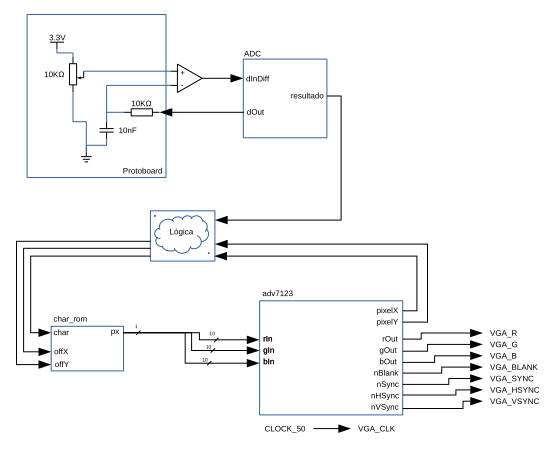
\includegraphics[width=10cm]{img/tp2.png}
\captionof{figure}{Diagrama de Bloques de componente tp2.}
\end{figure}

\section{Simulación y Verificación}

Escribí varios bancas de pruebas para probar la funcionalidad usando asserts, inspección de las ondas y los resultados. Por el componente ADV7123 usé SystemVerilog con un \textit{module}, un \textit{program} y el comando \textit{bind} para conectar el program a mi componented de VHDL. En el \textit{program} tengo algunos asserts y capturo las señales hsync, vsync, r, g, b, y les escribo a un archivo texto. Ese archivo puedo usar con el \href{https://ericeastwood.com/lab/vga-simulator/}{VGA Simulator}.

\begin{figure}[!h]
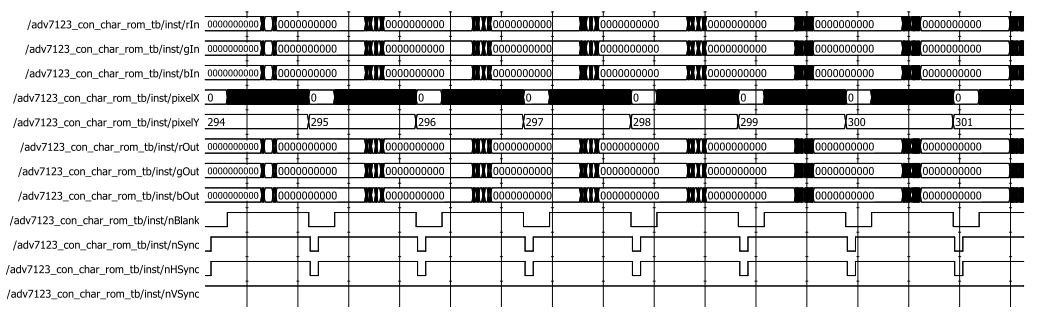
\includegraphics[width=12cm]{img/adv7123.png}
\captionof{figure}{Ondas de ADV7123.}
\end{figure}

\begin{figure}[!h]
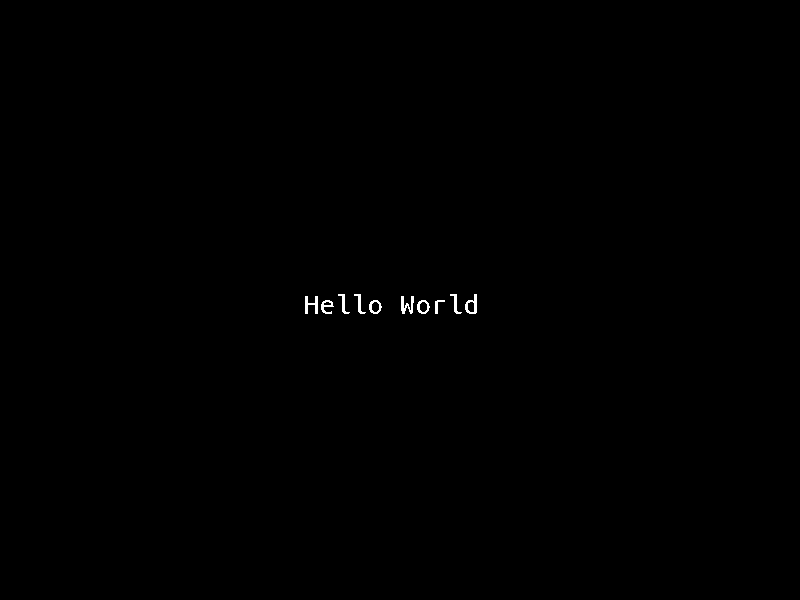
\includegraphics[width=12cm]{img/helloWorld.png}
\captionof{figure}{Resultado del banco de prueba adv7123\_con\_char\_rom.}
\end{figure}

\section{Síntesis}

He usado Quartus II para sintetizar el diseño.

\subsection{Resumen de síntesis}
\begin{tabular}{| l | r | r | r|}
\hline
\textbf{Ítem} & \textbf{Utilizado} & \textbf{Disponible} & \textbf{Porcentaje Utilizado} \\ \hline
Logic Elements & 266 & 33,216 & \textless 1\% \\
Registers & 148 & 33,216 & \textless 1\% \\ 
Bits de memoria & 45,600 & 483,840 & 9\% \\ 
Global Clocks & 1 & 16 & 6\% \\ \hline
\end{tabular} \\

TimeQuest Timing Analyzer me informe que el frecuencia máxima de reloj a la que está operable el circuito es 81.6MHz.

\section{Código}

Todo el código es disponible en mi github: \url{https://github.com/andrewparlane/fiuba6617/tree/master/TP2}.

\end{document}
